%%
%% pMMC Application Note — ECCB 2026 Proceedings
%% Uses OUP authoring template (oup-authoring-template.cls)
%%

%%%TRADITIONAL — matches Bioinformatics journal style (cudaMMC 2023)%%%
\documentclass[webpdf,traditional,large]{oup-authoring-template}%

\usepackage{newtxtext,newtxmath}
\graphicspath{{figures/}}

%%% Override OUP section formatting: left-aligned (matching published Bioinformatics style)
\makeatletter
\def\secsize{\fontsize{11.5bp}{11.75bp}\fontseries{b}\selectfont\raggedright}
\def\subsecsize{\fontsize{10.5bp}{11.75bp}\fontseries{b}\selectfont\raggedright}
\def\subsubsecsize{\fontsize{9.75bp}{11.75bp}\selectfont\bfseries\itshape\raggedright}
\def\paragraphsize{\fontsize{9.5bp}{11.75bp}\selectfont\bfseries\raggedright}
\makeatother

\begin{document}

\journaltitle{Bioinformatics}
\DOI{DOI added during production}
\copyrightyear{2026}
\pubyear{2026}
\vol{XX}
\issue{x}
\access{Published: Date added during production}
\appnotes{Application Note}

\firstpage{1}

\title[pMMC: GPU-accelerated Monte Carlo for 3D chromatin]{pMMC: fully GPU-accelerated multiscale Monte Carlo for three-dimensional chromatin structure reconstruction}

\author[1]{Mohammad Saqib}
\author[2]{Kaustav Sengupta}
\author[2,3,$\ast$]{Dariusz Plewczynski}

\address[1]{\orgdiv{Interdisciplinary Doctoral School}, \orgname{University of Warsaw}, \orgaddress{\state{Warsaw}, \country{Poland}}}
\address[2]{\orgdiv{Laboratory of Bioinformatics and Computational Genomics, Faculty of Mathematics and Information Science}, \orgname{Warsaw University of Technology}, \orgaddress{\state{Warsaw}, \country{Poland}}}
\address[3]{\orgdiv{Laboratory of Functional and Structural Genomics, Centre of New Technologies}, \orgname{University of Warsaw}, \orgaddress{\street{Banacha 2c Street}, \postcode{02-097}, \state{Warsaw}, \country{Poland}}}

\corresp[$\ast$]{Corresponding author. \href{email:d.plewczynski@cent.uw.edu.pl}{d.plewczynski@cent.uw.edu.pl}}

\received{March}{15}{2026}

\abstract{
\textbf{Motivation:} Reconstructing three-dimensional chromatin architecture from chromosome conformation capture data requires computationally demanding Monte Carlo simulations. The growing scale of modern ChIA-PET and Hi-C datasets, spanning entire genomes at kilobase resolution, has made existing tools insufficient for generating large structural ensembles within practical time frames. Both the original 3D-GNOME engine and its GPU-extended successor cudaMMC leave substantial portions of the modelling pipeline on the CPU, limiting overall throughput.\\
\textbf{Results:} We present pMMC, a fully GPU-accelerated reimplementation of the multiscale Monte Carlo chromatin modelling engine. pMMC transfers all three simulation stages --- heatmap-level territory positioning, interaction-arc-guided anchor refinement, and polymer-smoothing bead placement --- onto CUDA kernels, eliminating the CPU bottleneck that dominated execution time in cudaMMC. On a benchmark comprising CTCF-mediated ChIA-PET data for human chromosomes of varying sizes, pMMC achieves a 13.6-fold speed-up over 3D-GNOME and a 1.5-fold speed-up over cudaMMC for the largest chromosome tested, while producing structurally equivalent output (Pearson $r = 1.000$ for distance matrices). Across all 22 autosomes and chromosome~X on the GRCh38 assembly, pMMC demonstrates near-constant wall-clock time regardless of chromosome size, whereas cudaMMC exhibits size-dependent scaling. Ensemble modelling of 50 structures for chromosome~1 shows that pMMC yields higher inter-model consistency (median Spearman $\rho = 0.86$ vs.\ $0.59$ for cudaMMC). The tool supports HCM, mmCIF, and PDB output formats and is freely available as open-source software.\\
\textbf{Availability and implementation:} Source code, benchmark data, and documentation are available at \url{https://github.com/SFGLab/pMMC}. pMMC is implemented in C++17/CUDA and builds on Linux with CMake.\\
\textbf{Contact:} \href{email:d.plewczynski@cent.uw.edu.pl}{d.plewczynski@cent.uw.edu.pl}}

\keywords{3D genome, chromatin structure, Monte Carlo, CUDA, GPU, ChIA-PET}

\maketitle

%% =====================================================================
%% 1. INTRODUCTION
%% =====================================================================

\section{Introduction}

The spatial organisation of chromatin inside the cell nucleus plays a fundamental role in gene regulation, DNA replication, and repair processes \citep{Szalaj2018organization}. Chromosome conformation capture techniques such as Hi-C and ChIA-PET have provided increasingly detailed maps of chromatin contacts, revealing a hierarchy of structural features from chromosome territories through topologically associating domains down to individual loops mediated by proteins such as CTCF \citep{Fudenberg2016loop, Nuebler2018chromatin}. Computational approaches that translate these pairwise interaction frequencies into three-dimensional polymer models are therefore essential for interpreting the biological consequences of genome architecture \citep{Chiariello2016polymer, Tjong2016population}.

Several reconstruction methods have been proposed, ranging from probabilistic frameworks based on Markov chain Monte Carlo sampling \citep{Rousseau2011chromatin} to energy-based polymer models \citep{Korsak2024multimm, Korsak2024loopsage}. Among these, the 3D-GNOME engine \citep{Szalaj2016engine} introduced a multiscale Monte Carlo strategy with simulated annealing that operates hierarchically: first positioning chromosome territories and megabase-scale segments using contact frequency heatmaps, then refining anchor positions based on interaction arcs, and finally generating kilobase-resolution bead chains by polymer smoothing. The 3D-GNOME web server \citep{Szalaj2016gnome, Wlasnowolski2023gnome} makes this pipeline accessible to the community, but its CPU-oriented implementation becomes a bottleneck when modelling large chromosomes or generating statistical ensembles of hundreds of structures.

To address this limitation, cudaMMC \citep{Wlasnowolski2023cudammc} moved the heatmap-level Monte Carlo stage onto an NVIDIA GPU, achieving substantial speed-ups over the original 3D-GNOME. However, cudaMMC still executes the arc-level and smoothing-level simulations on the CPU, and for large chromosomes these stages account for the majority of the total runtime. Moreover, cudaMMC allocates and deallocates GPU resources on every kernel invocation, introducing overhead that scales with the number of segments. GPU-based Monte Carlo sampling has been shown to provide substantial acceleration for polymer simulations in other contexts \citep{Lee2010gpu, Gross2011parallel}, motivating a more comprehensive GPU approach to genome structure modelling.

In this work we present pMMC, a comprehensive GPU-accelerated reimplementation that transfers all three Monte Carlo stages onto CUDA kernels, caches GPU resources across invocations, and applies algorithmic refinements to convergence detection. The result is a tool that runs the entire modelling pipeline on the GPU with near-constant wall-clock time regardless of chromosome size, while maintaining full structural equivalence with cudaMMC outputs.

%% =====================================================================
%% 2. MATERIALS AND METHODS
%% =====================================================================

\section{Materials and methods}

\subsection{3D-GNOME --- CPU-oriented approach}

The original 3D-GNOME modelling engine \citep{Szalaj2016engine} reconstructs chromatin structure through a top-down multiscale approach. In the first stage, the chromosome is partitioned into approximately 2\,Mb segments based on interaction patterns, and Monte Carlo simulated annealing is used to position segment-level beads by minimising an energy function derived from singleton contact frequency heatmaps. In the second stage, anchor positions within each segment are refined independently by matching interaction arc distances obtained from PET cluster counts. The third stage generates sub-anchor beads between adjacent anchors, imposing polymer spring constraints on stretch, compression, and bending angle to produce a smooth fibre path. All three stages run entirely on the CPU, and the Monte Carlo phases are executed sequentially for every interaction block within every segment.

\subsection{cudaMMC approach --- GPU-extended}

\citet{Wlasnowolski2023cudammc} accelerated the heatmap-level Monte Carlo stage by offloading it to an NVIDIA GPU. The parallelisation strategy launches multiple CUDA warps, where each warp of 32 cooperative threads runs an independent simulated annealing trajectory. Within each warp, threads propose random bead displacements and cooperatively evaluate the energy change through warp-level reduction, selecting the best candidate at each step. This design avoids global synchronisation barriers and provides a substantial speed-up over the CPU implementation for the coarsest modelling level.

However, the arc-level and smoothing-level stages in cudaMMC continue to run on the CPU. Because these stages iterate over every segment independently and each invocation involves allocating and releasing GPU memory for random number generator states and working buffers, overhead accumulates in proportion to chromosome size. For the largest human chromosome, which contains over 100 segments and triggers approximately 284 separate kernel invocations, the CPU-bound phases dominate the total execution time.

\subsection{pMMC approach --- GPU-oriented, optimised, and additional features}

pMMC extends the GPU parallelisation to all three Monte Carlo stages and introduces several architectural improvements. The key design is illustrated in Figure~\ref{fig:pipeline}.

\begin{figure}[!t]%
\centering

\includegraphics[width=\columnwidth]{pipeline.pdf}
\caption{Pipeline of the pMMC fully GPU-accelerated multiscale Monte Carlo algorithm for chromatin 3D structure reconstruction. Input ChIA-PET data are parsed into a four-level hierarchical tree. Three successive CUDA kernel stages refine the structure from coarse territory placement to fine-grained polymer smoothing. A persistent GPU resource cache eliminates per-segment allocation overhead, and a composite energy function guides the simulated annealing at each level.}\label{fig:pipeline}
\end{figure}

\textit{Fully GPU-resident simulation.} The arc-level and smoothing-level Monte Carlo loops, which previously ran on the CPU in cudaMMC, are now implemented as dedicated CUDA kernels. Each kernel launches one block per streaming multiprocessor with 128 threads per block, organised as four independent warps per block. Each warp runs a complete simulated annealing trajectory, with one thread proposing bead displacements and all 32 threads cooperating on energy evaluation via warp-shuffle reduction. A hard iteration cap prevents any kernel from running indefinitely in pathological convergence cases.

\textit{Persistent GPU resource caching.} Rather than allocating and freeing GPU random-number generator states and working buffers for every segment, pMMC maintains a persistent cache that is initialised once at programme startup and reused throughout the modelling run. This eliminates the per-segment allocation overhead that dominated wall-clock time for large chromosomes in cudaMMC. For chromosome~1, which contains 125 segments and triggers approximately 284 kernel invocations, the cumulative allocation savings are substantial.

\textit{Refined convergence detection.} The original stop condition in cudaMMC relied solely on temperature decay, which could require over 250\,000 iterations before triggering. pMMC introduces milestone-based convergence detection with a configurable iteration budget that terminates the simulated annealing when score improvement stalls, balancing convergence quality against computational cost.

\textit{Additional capabilities.} Beyond performance improvements, pMMC provides several features not present in cudaMMC: multidimensional scaling initialisation of bead positions as an alternative to random placement, deterministic seeding for reproducible results across runs, export of reconstructed structures in mmCIF and PDB formats in addition to the native hierarchical format, a built-in benchmarking pipeline with synthetic data generation and structural comparison metrics (RMSD, Pearson correlation, stratum-adjusted correlation), memory budget enforcement with graceful shutdown, and the ability to reconstruct arbitrary genomic sub-regions rather than only whole chromosomes.

\subsection{Chromatin interaction data}

We evaluated all three tools --- the original 3D-GNOME (denoted 3dome\_mmc), cudaMMC, and pMMC --- on CTCF-mediated ChIA-PET interaction data for the GM12878 lymphoblastoid cell line. The primary benchmark uses data for chromosomes~1, 14, and 21, which represent large, medium, and small chromosomes respectively (125, 54, and 25 segments; 84\,385, 29\,641, and 7\,825 chromatin loops). A secondary scalability benchmark uses data for all 22 autosomes and chromosome~X mapped to the GRCh38 reference assembly to assess how each tool scales with chromosome size. All experiments were conducted on a workstation equipped with an NVIDIA RTX~4070 GPU (Ada Lovelace architecture, 46 streaming multiprocessors, 12\,GB VRAM) and an AMD Ryzen~7 CPU with 32\,GB RAM. Each tool used equivalent simulated annealing schedules and the same input data.

%% =====================================================================
%% 3. COMPARISON OF PERFORMANCE
%% =====================================================================

\section{Comparison of performance between pMMC vs cudaMMC and 3D-GNOME}

We benchmarked all three tools using 10 replicate runs per tool per chromosome on the primary dataset, with GPU utilisation and memory monitored continuously.

\paragraph{Wall-clock time.}
Table~\ref{tab:walltime} reports mean wall-clock times and coefficients of variation. For chromosome~1 (the largest, with 125 segments), pMMC completed modelling in 4.92\,s on average, compared with 7.49\,s for cudaMMC and 67.0\,s for 3D-GNOME. This corresponds to a 13.6$\times$ speed-up over 3D-GNOME and a 1.52$\times$ speed-up over cudaMMC. For chromosome~14 (54 segments), the speed-ups were 3.4$\times$ and 1.23$\times$, respectively. For chromosome~21 (25 segments), the differences were smaller (1.15$\times$ and 1.07$\times$), as the reduced number of segments leaves less room for gains from the GPU-accelerated arc and smoothing phases. Notably, pMMC's wall-clock time varies only modestly across chromosomes of very different sizes (4.92\,s for chr1 versus 3.96\,s for chr21), whereas 3D-GNOME's time increases more than 14-fold over the same range. The coefficient of variation was below 8\% for all tools across all chromosomes, indicating stable and reproducible performance.

\begin{table}[!t]
\begin{center}
\begin{minipage}{\columnwidth}
\caption{Mean wall-clock time (seconds) and coefficient of variation (CV) over 10 replicate runs.\label{tab:walltime}}%
\tabcolsep=3pt
\begin{tabular*}{\columnwidth}{@{\extracolsep\fill}lrrrrrr@{\extracolsep\fill}}
\toprule
 & \multicolumn{2}{c}{chr1 (125\,seg)} & \multicolumn{2}{c}{chr14 (54\,seg)} & \multicolumn{2}{c}{chr21 (25\,seg)} \\
\cline{2-3}\cline{4-5}\cline{6-7}
Tool & Time\,(s) & CV & Time\,(s) & CV & Time\,(s) & CV \\
\midrule
3D-GNOME  & 67.0\,(1.1) & .016 & 14.7\,(0.6) & .038 & 4.56\,(0.3) & .056 \\
cudaMMC   &  7.49\,(0.3) & .042 &  5.27\,(0.3) & .064 & 4.24\,(0.3) & .078 \\
pMMC      &  4.92\,(0.3) & .062 &  4.27\,(0.3) & .062 & 3.96\,(0.3) & .068 \\
\botrule
\end{tabular*}
\end{minipage}
\end{center}
\end{table}

Figure~\ref{fig:combined}(a) shows the wall-clock time distribution across chromosomes, and Figure~\ref{fig:combined}(b) presents the speedup factors of pMMC relative to both cudaMMC and 3D-GNOME. The speedup of pMMC over cudaMMC grows with chromosome size, reflecting the increasing dominance of the CPU-bound arc and smoothing phases in cudaMMC for chromosomes with many segments.

\begin{figure*}[!t]%
\centering
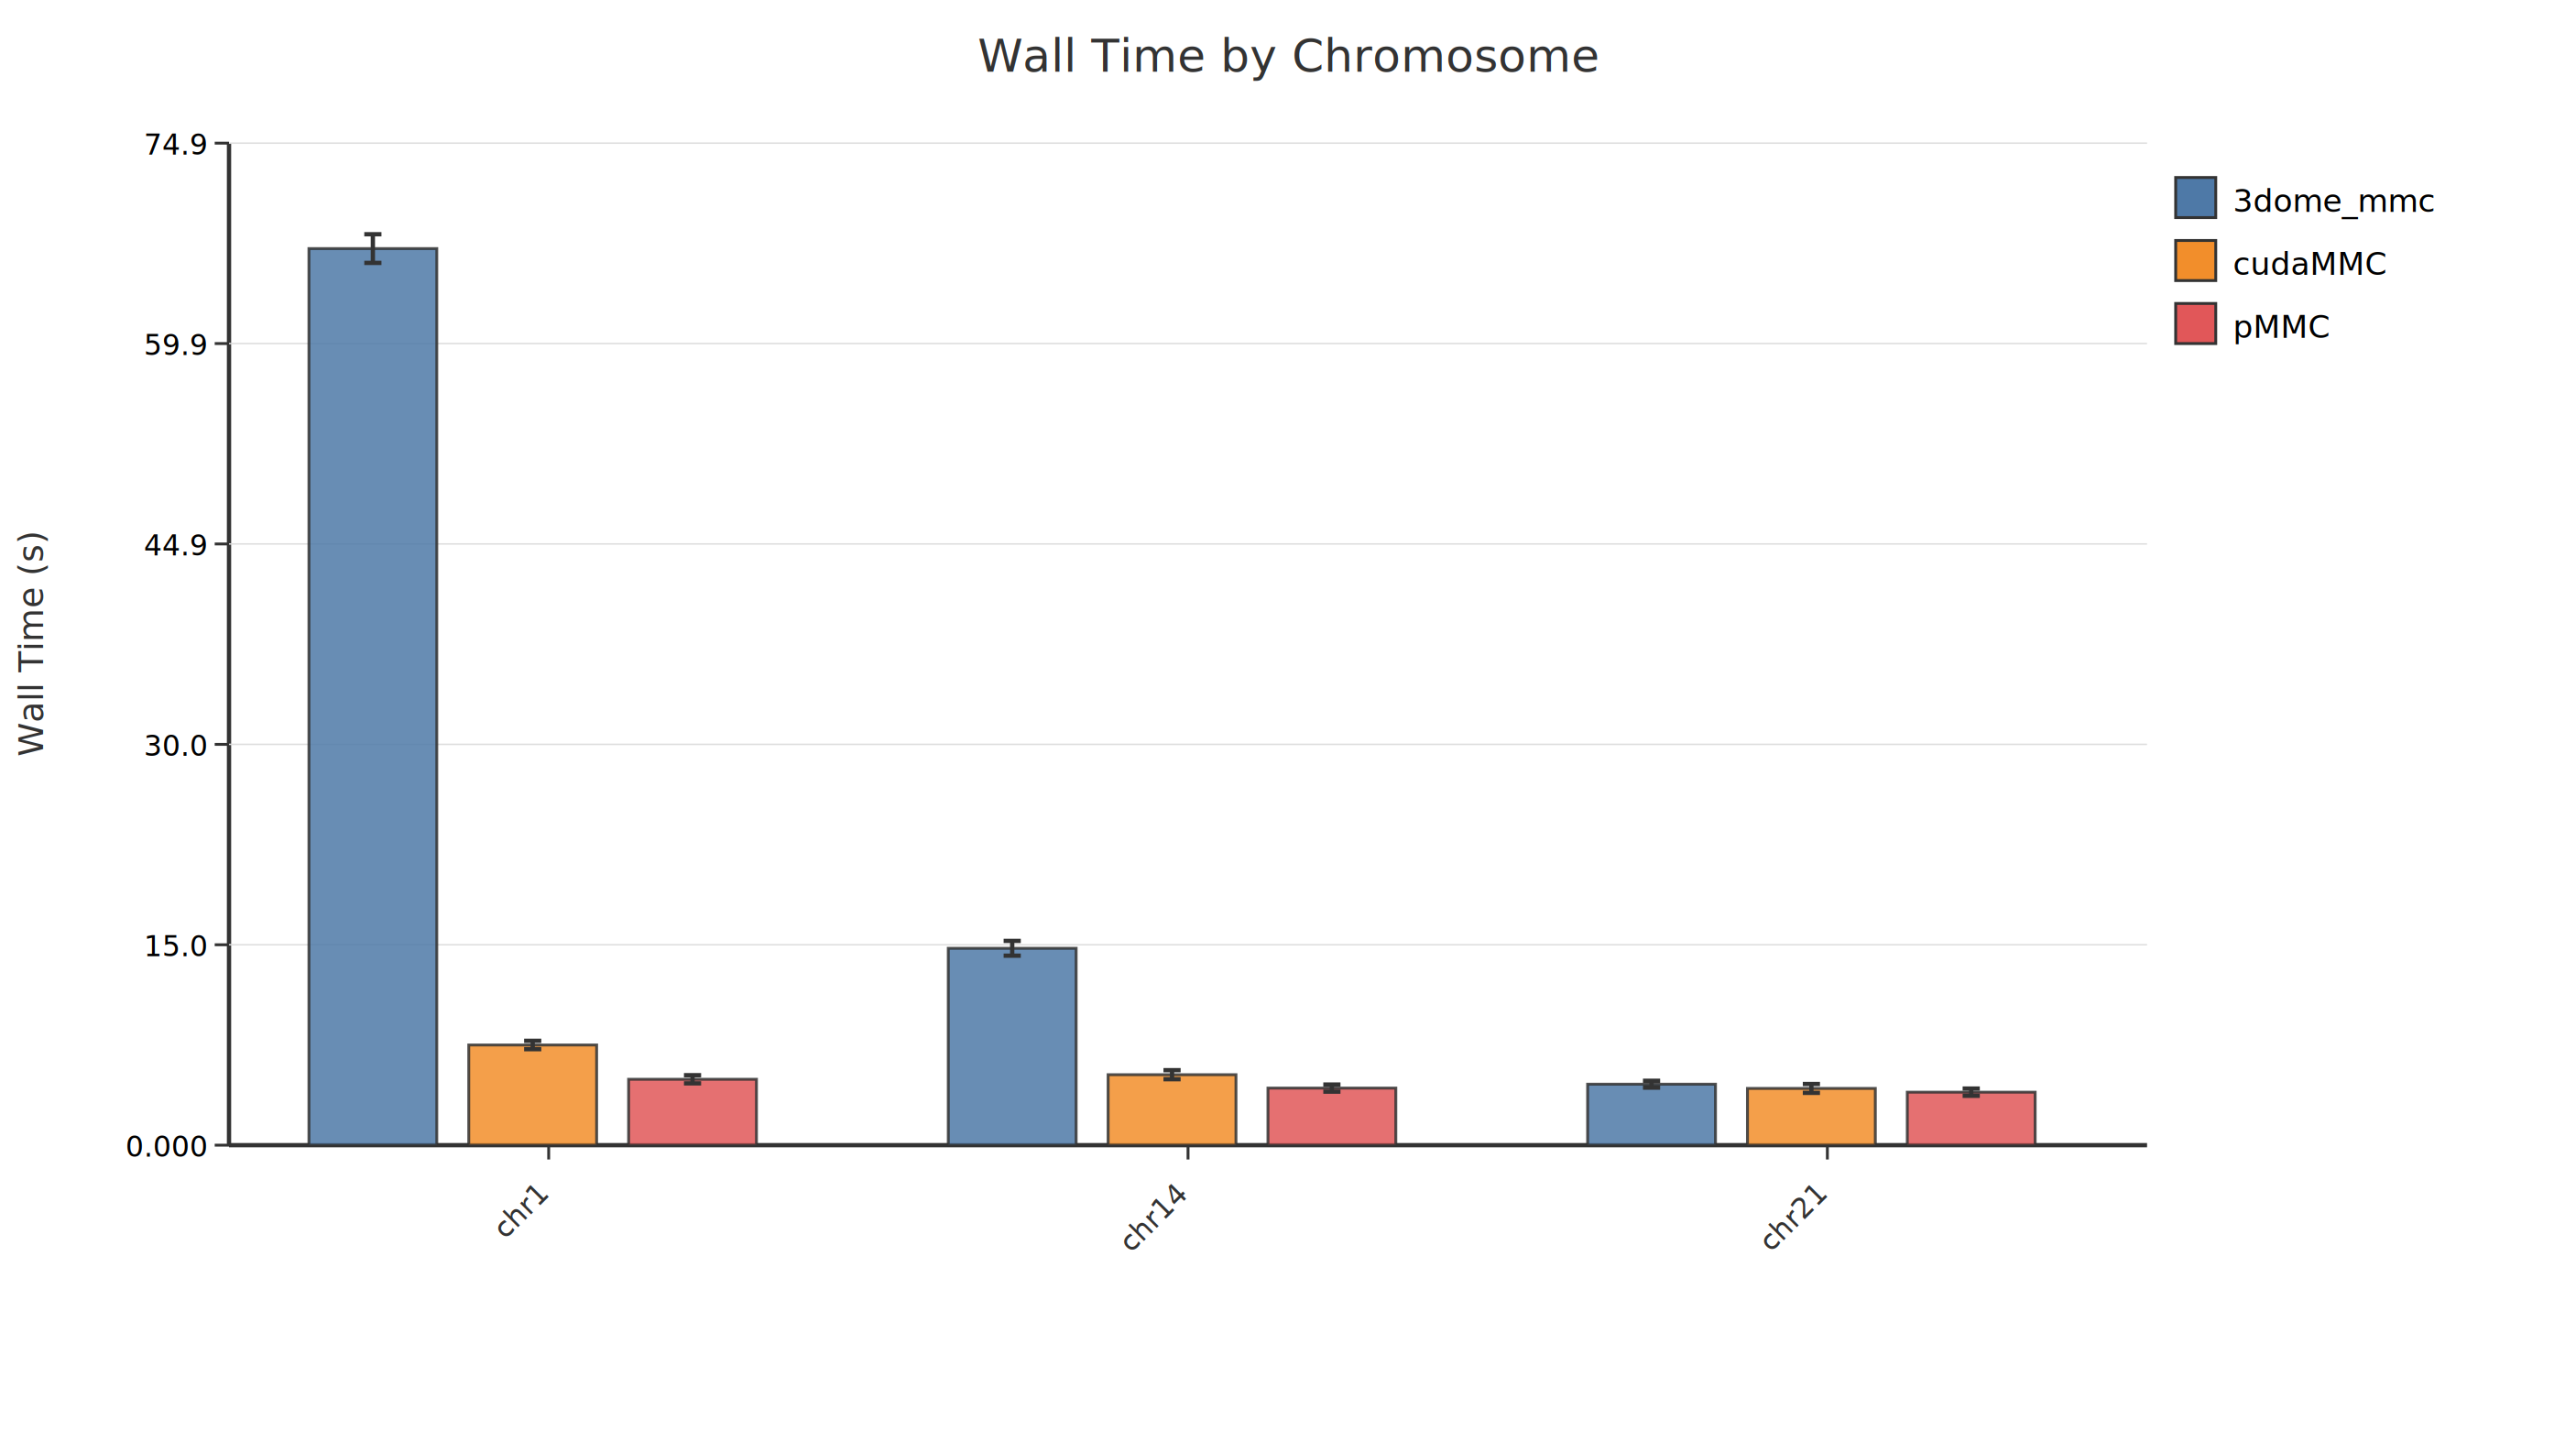
\includegraphics[width=0.48\textwidth]{wall_time_by_chromosome.png}\hfill
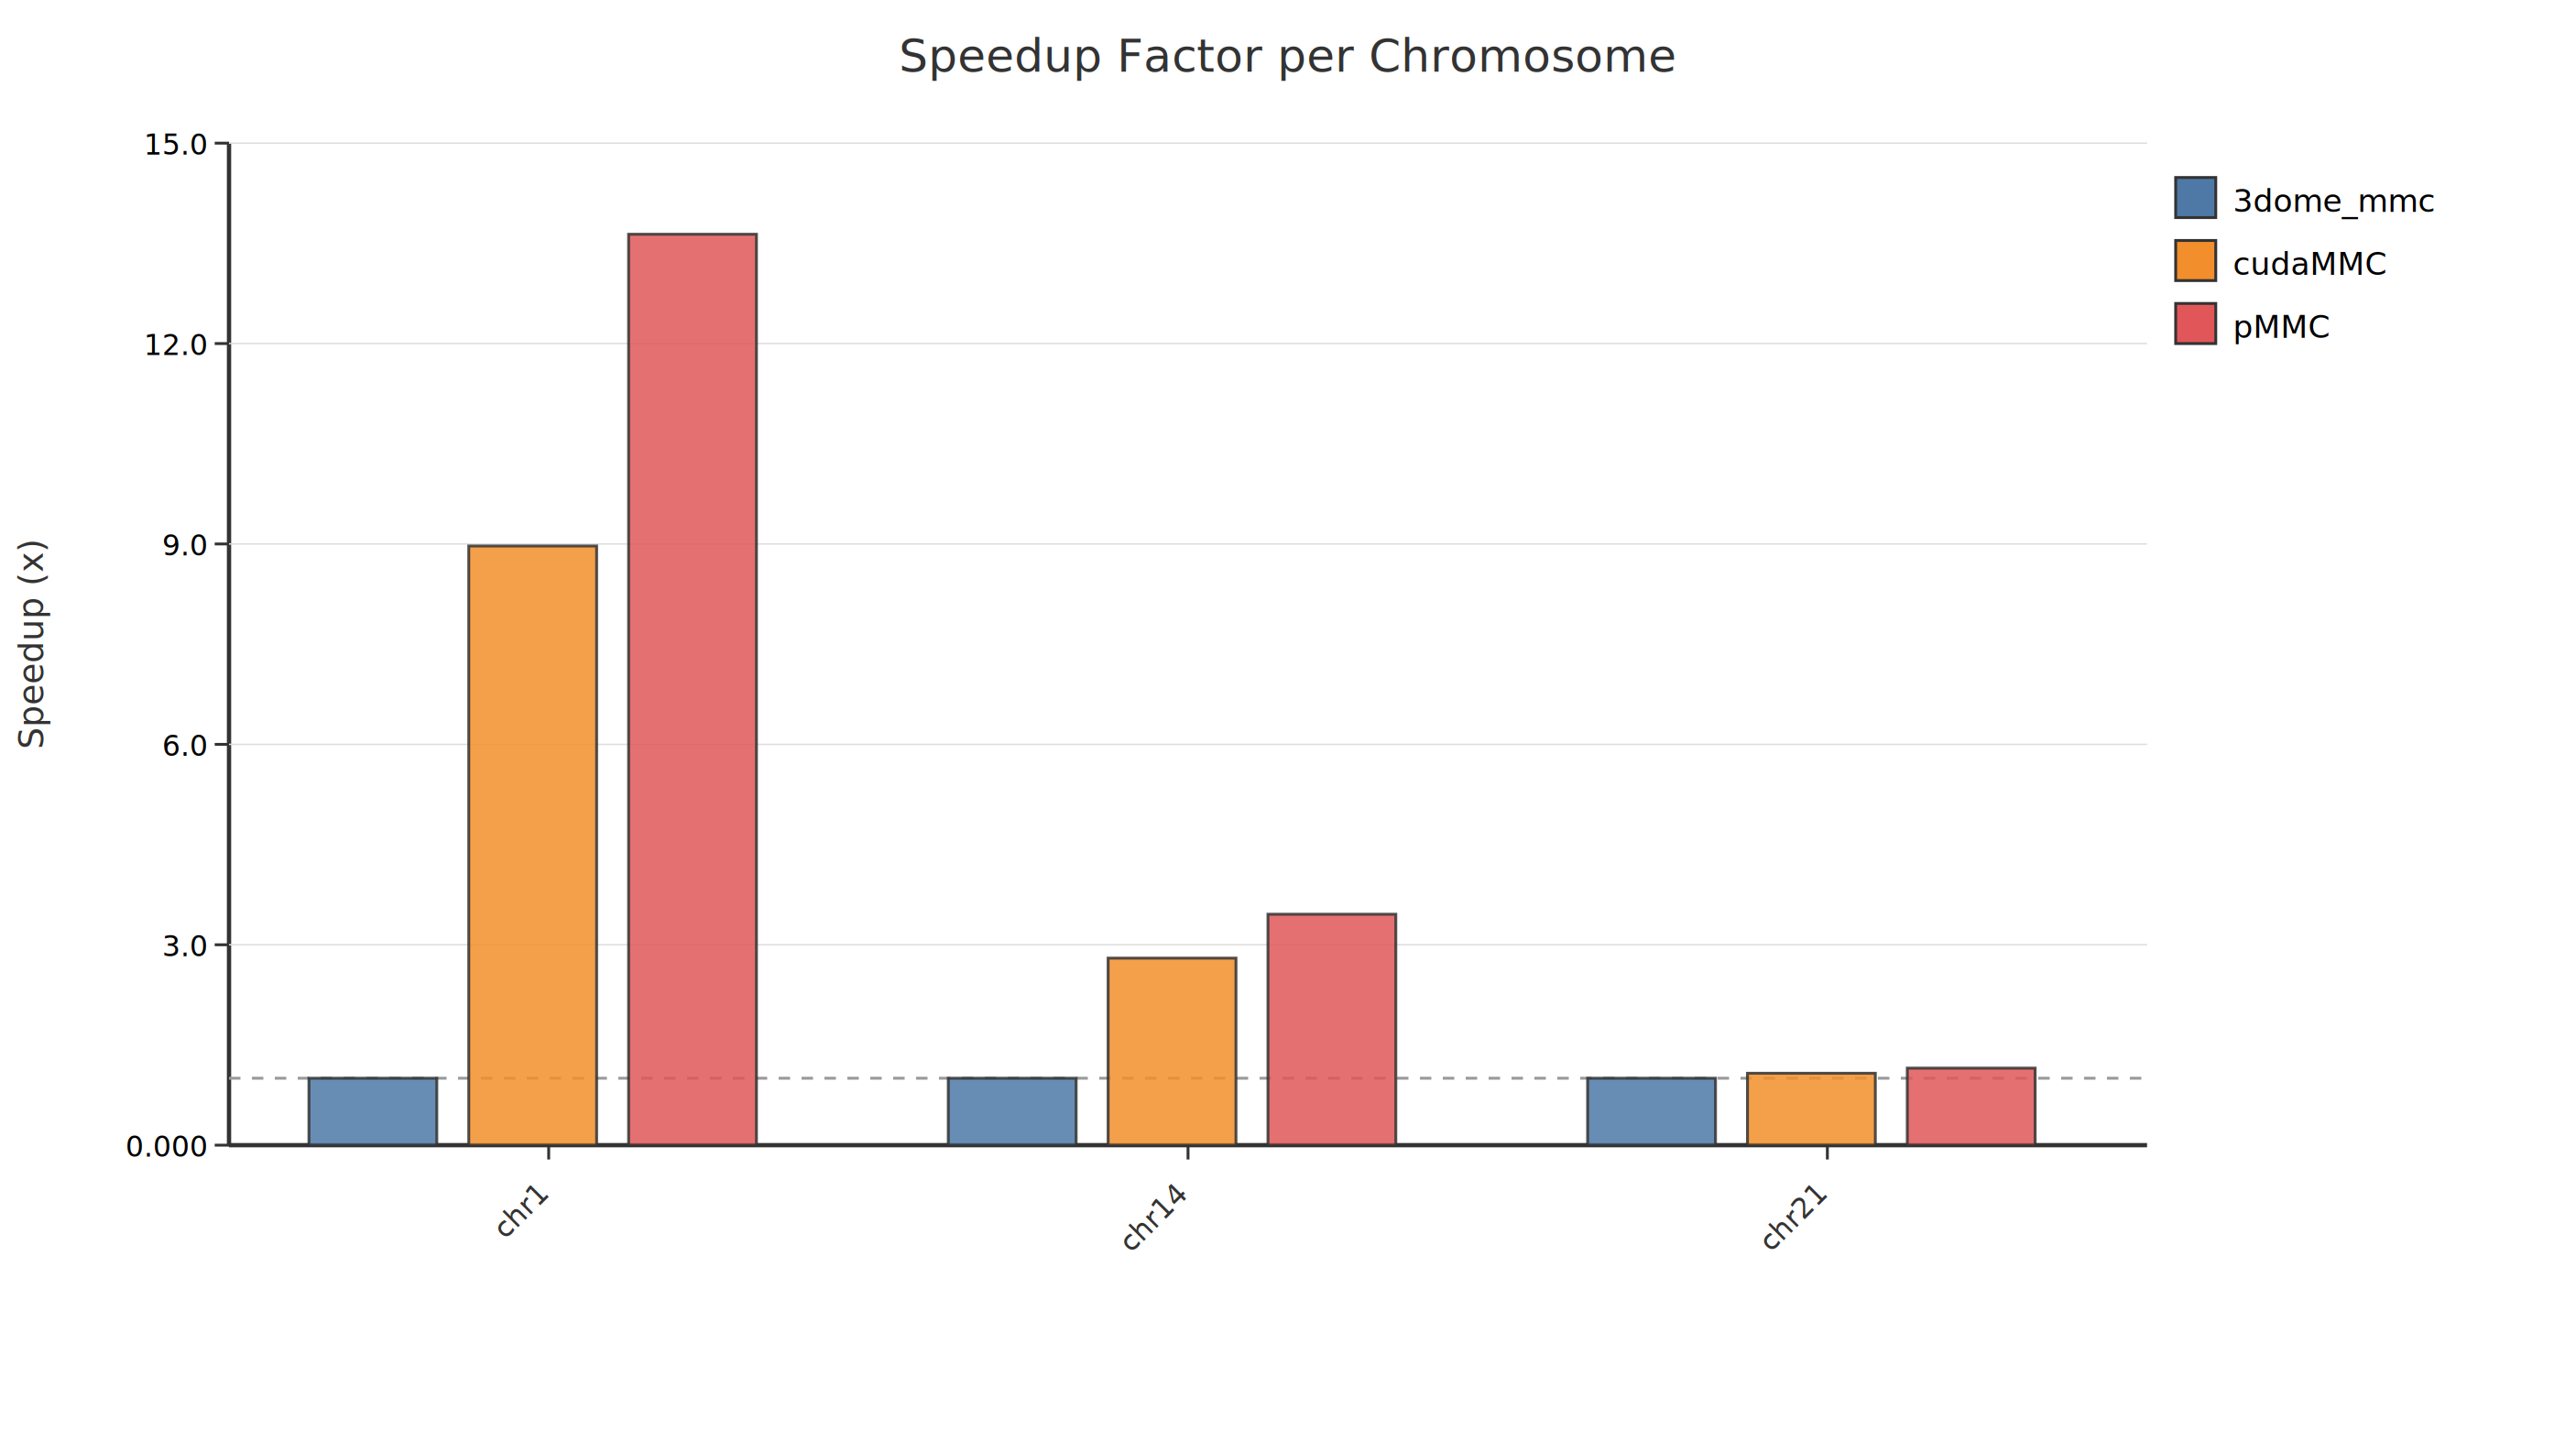
\includegraphics[width=0.48\textwidth]{speedup_factor.png}
\caption{(a)~Wall-clock time by chromosome for the three tools across 10 replicate runs. (b)~Speedup factor of pMMC relative to cudaMMC and 3D-GNOME, shown per chromosome. Error bars indicate standard deviation across 10 runs.}\label{fig:combined}
\end{figure*}

\paragraph{Scalability.}
Figure~\ref{fig:scaling}(a) shows the scaling regression of wall-clock time against the number of segments. The ratio of chr1 to chr21 wall time reveals the scaling behaviour: 3D-GNOME exhibits a ratio of 14.7$\times$, cudaMMC 1.77$\times$, and pMMC 1.24$\times$. The near-flat profile of pMMC indicates that its runtime is dominated by a fixed overhead (GPU initialisation, I/O) rather than by computation that scales with the number of interaction blocks. The secondary scalability benchmark across all GRCh38 chromosomes (Figure~\ref{fig:scaling}(b)) confirms this advantage at genome scale: pMMC maintains a near-constant execution time of approximately 4--5\,s regardless of chromosome size, while cudaMMC's median wall time rises from approximately 4.5\,s for small chromosomes to over 8\,s for chromosome~1. This characteristic makes pMMC especially suitable for whole-genome reconstruction, where many large chromosomes must be processed with predictable, uniform per-chromosome cost.

\begin{figure*}[!t]%
\centering
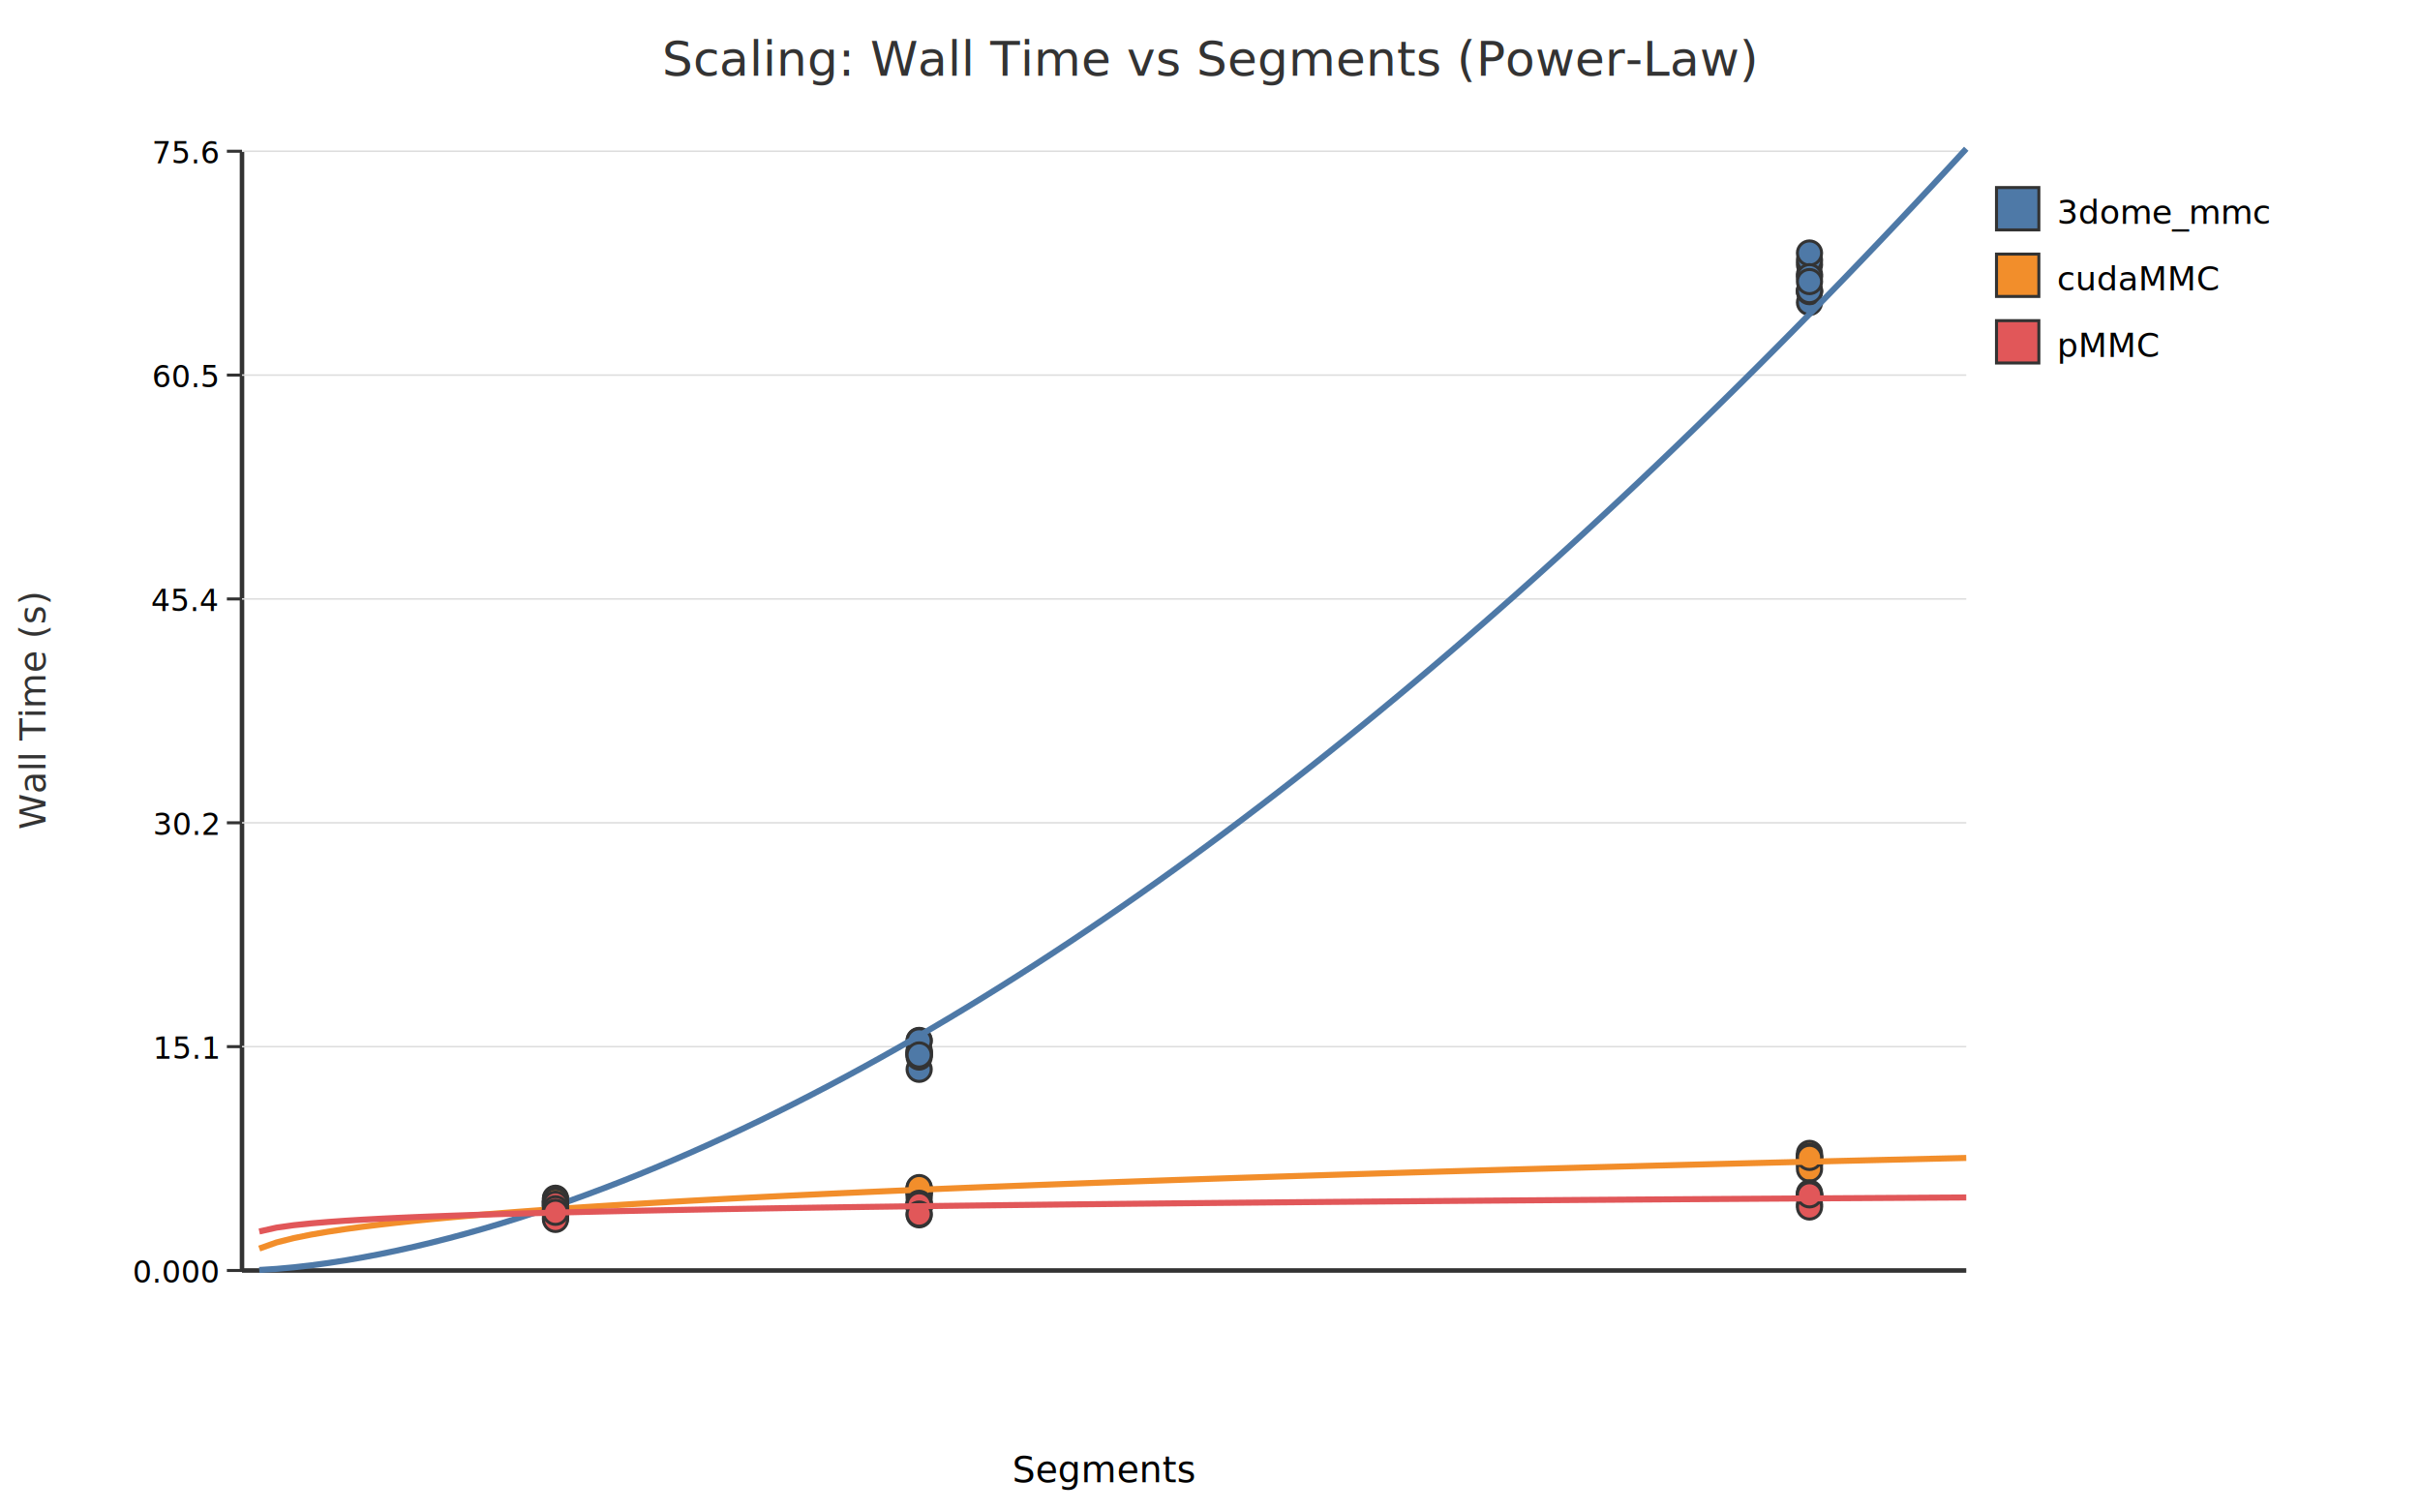
\includegraphics[width=0.48\textwidth]{scaling_regression.png}\hfill
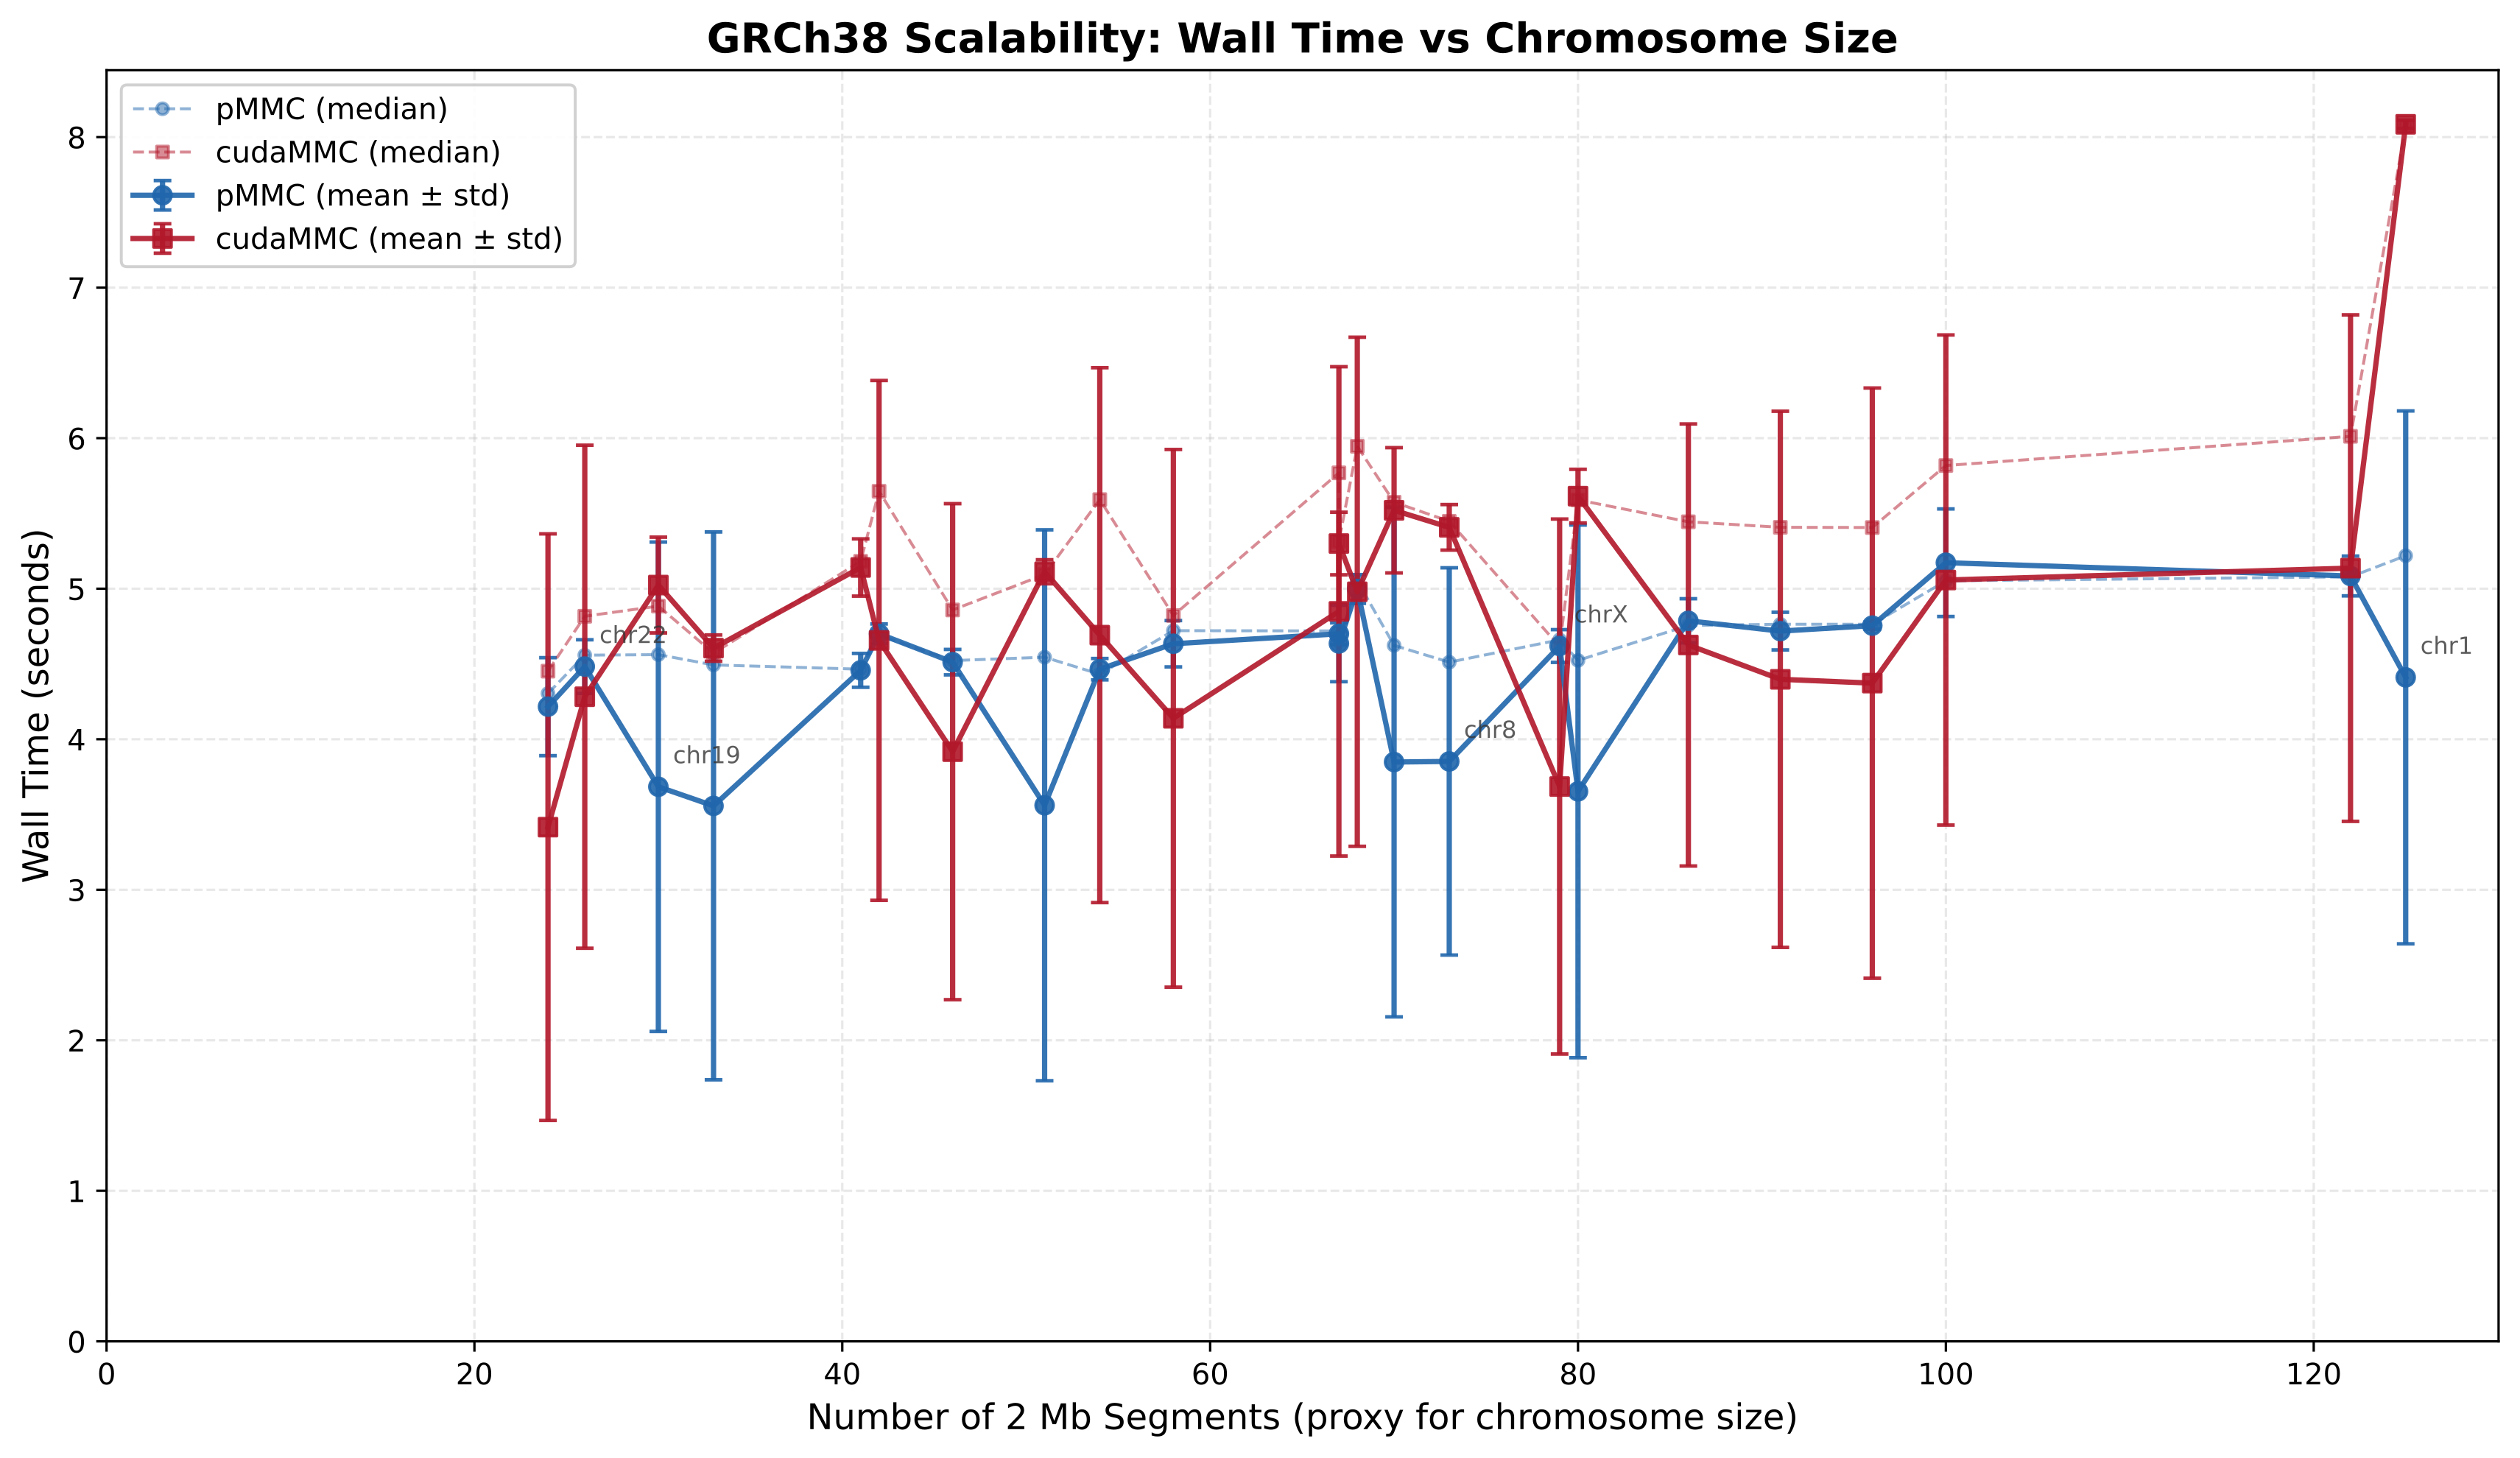
\includegraphics[width=0.48\textwidth]{scalability_grch38.png}
\caption{(a)~Scaling regression of wall-clock time vs.\ number of segments for the primary benchmark. (b)~Scalability comparison across all human autosomes and chromosome~X on GRCh38 data (3 runs per chromosome). pMMC (blue) maintains near-constant wall-clock time regardless of chromosome size, whereas cudaMMC (red) exhibits size-dependent scaling.}\label{fig:scaling}
\end{figure*}

\paragraph{Output quality.}
The pairwise Pearson correlation of distance matrices between pMMC and cudaMMC outputs was $r = 1.000$ for all three chromosomes (chr1, chr14, chr21), confirming that pMMC produces structurally equivalent output when the same random seed is used. Intra-tool consistency was also $r = 1.000$ for pMMC across different runs with the same seed, demonstrating full deterministic reproducibility. Figure~\ref{fig:quality}(a) shows the output quality heatmap. Beyond single-model equivalence, we assessed structural consistency across 50-model ensembles for chromosome~1. The median pairwise Spearman correlation of distance matrices was $\rho = 0.86$ for pMMC ensembles versus $\rho = 0.59$ for cudaMMC (Figure~\ref{fig:similarity}), indicating that pMMC produces more structurally coherent model populations. This higher consistency suggests that the refined convergence criteria and fully GPU-resident optimisation allow pMMC's simulated annealing to explore the energy landscape more efficiently, converging to a tighter region of conformational space.

\begin{figure*}[!t]%
\centering
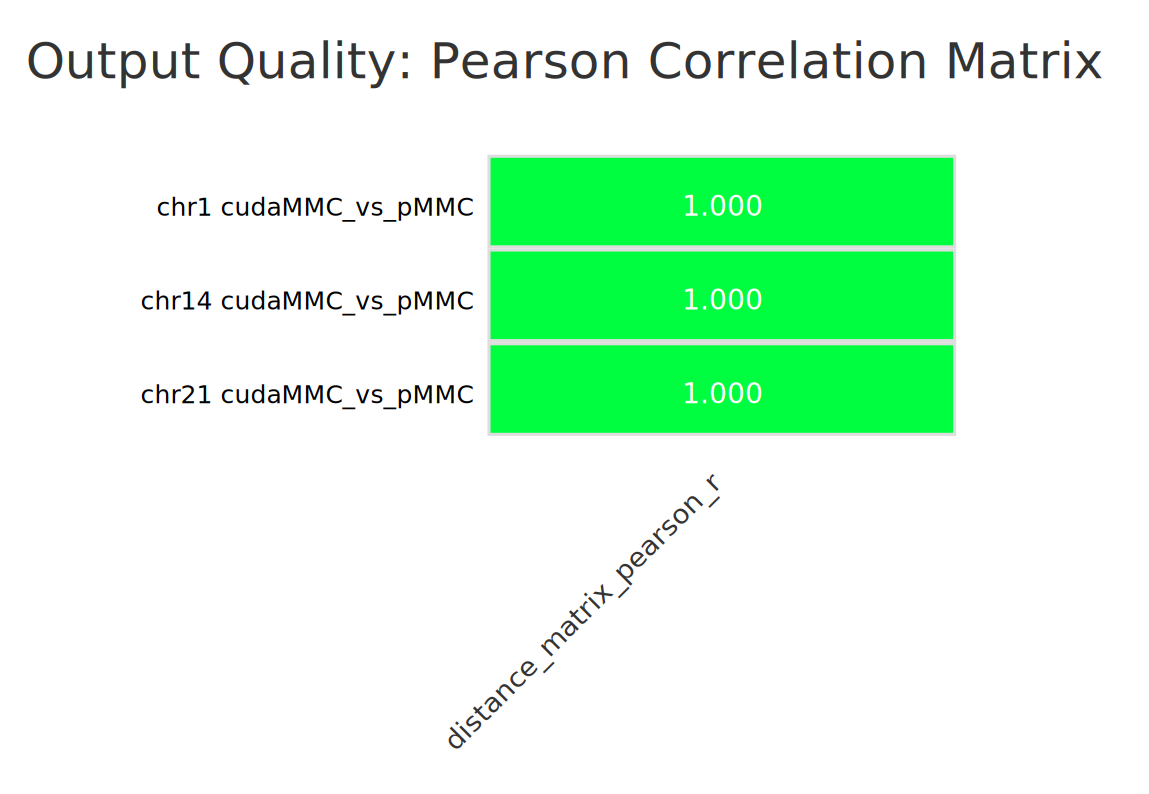
\includegraphics[width=0.48\textwidth]{output_quality_heatmap.png}\hfill
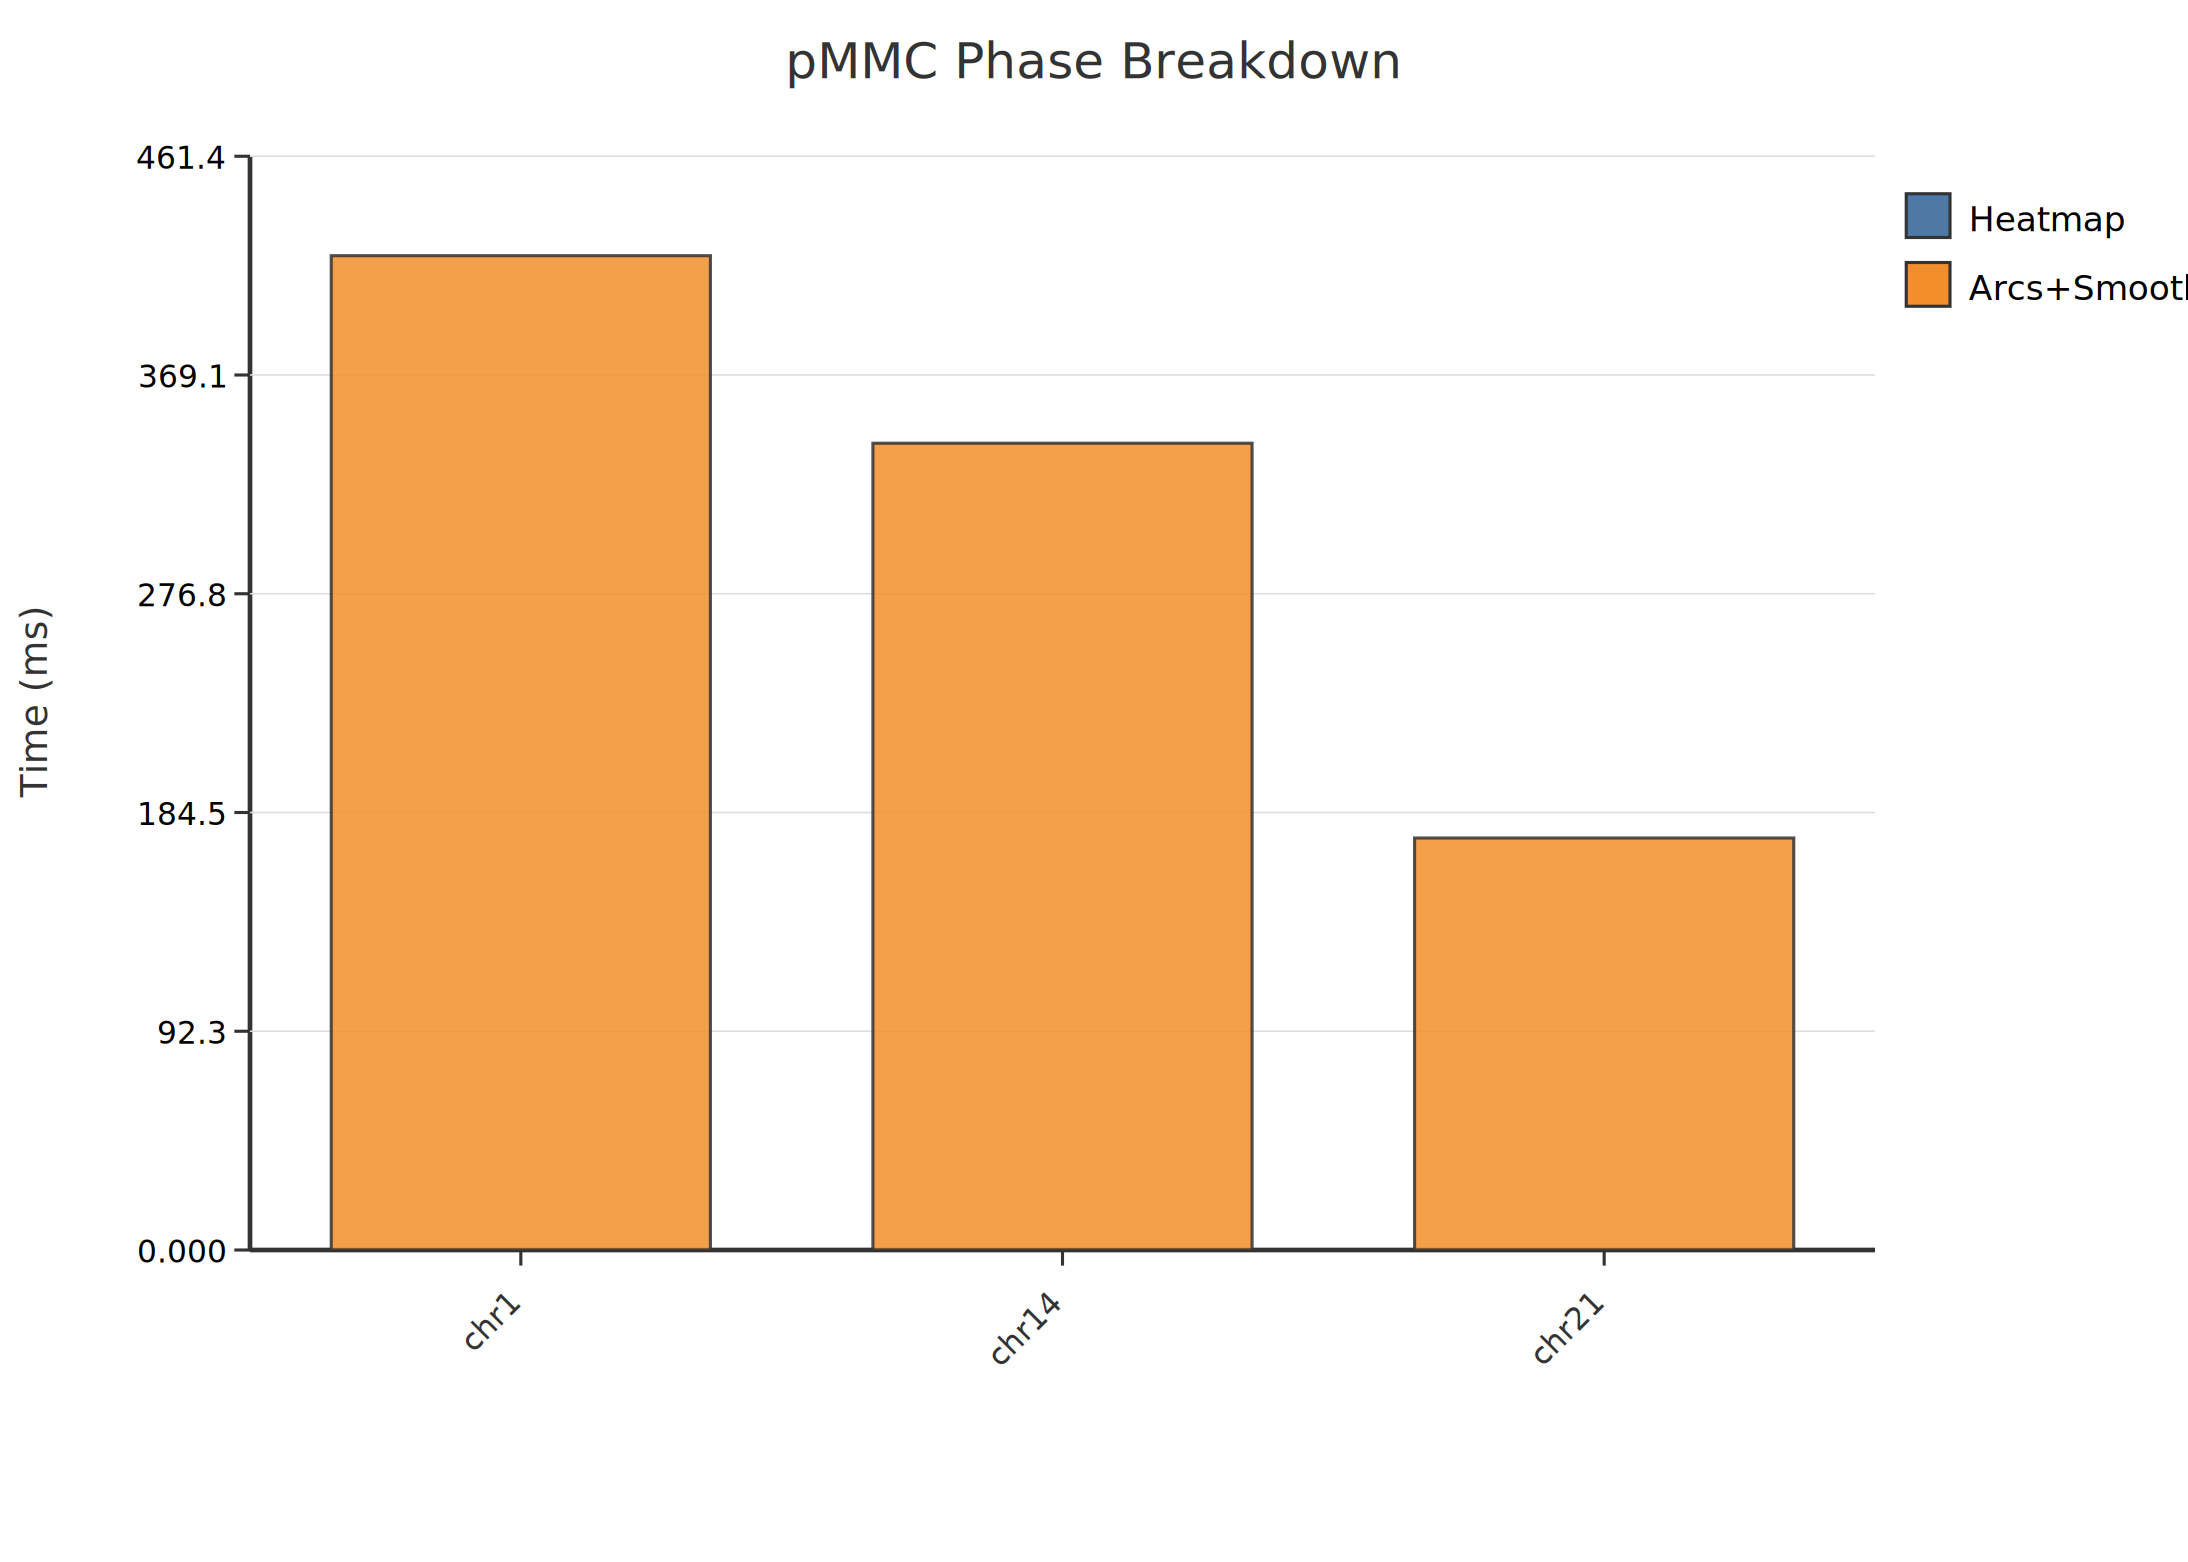
\includegraphics[width=0.48\textwidth]{phase_breakdown.png}
\caption{(a)~Output quality heatmap: Pearson correlation of pairwise distance matrices between tools and across chromosomes. (b)~Phase breakdown showing time distribution across Monte Carlo phases for each tool, illustrating how pMMC shifts the computational burden from CPU to GPU.}\label{fig:quality}
\end{figure*}

\paragraph{Ensemble modelling.}
Ensemble modelling is particularly relevant for statistical analyses of chromatin conformation, for instance when assessing how structural variants alter distances between gene promoters and enhancers \citep{Wlasnowolski2023gnome}. We generated ensembles of 50 models per chromosome, averaged over 3 independent ensemble runs. For chromosome~1, pMMC generated the entire ensemble in 243\,s (roughly 4 minutes), compared with 375\,s for cudaMMC and 3307\,s (55 minutes) for 3D-GNOME. This corresponds to speedups of 1.54$\times$ over cudaMMC and 13.6$\times$ over 3D-GNOME at ensemble scale. For chromosome~14, the ensemble times were 228\,s (pMMC), 280\,s (cudaMMC), and 743\,s (3D-GNOME). For chromosome~21, all tools performed similarly: 205\,s (pMMC), 211\,s (cudaMMC), and 224\,s (3D-GNOME).

\begin{figure}[!t]%
\centering
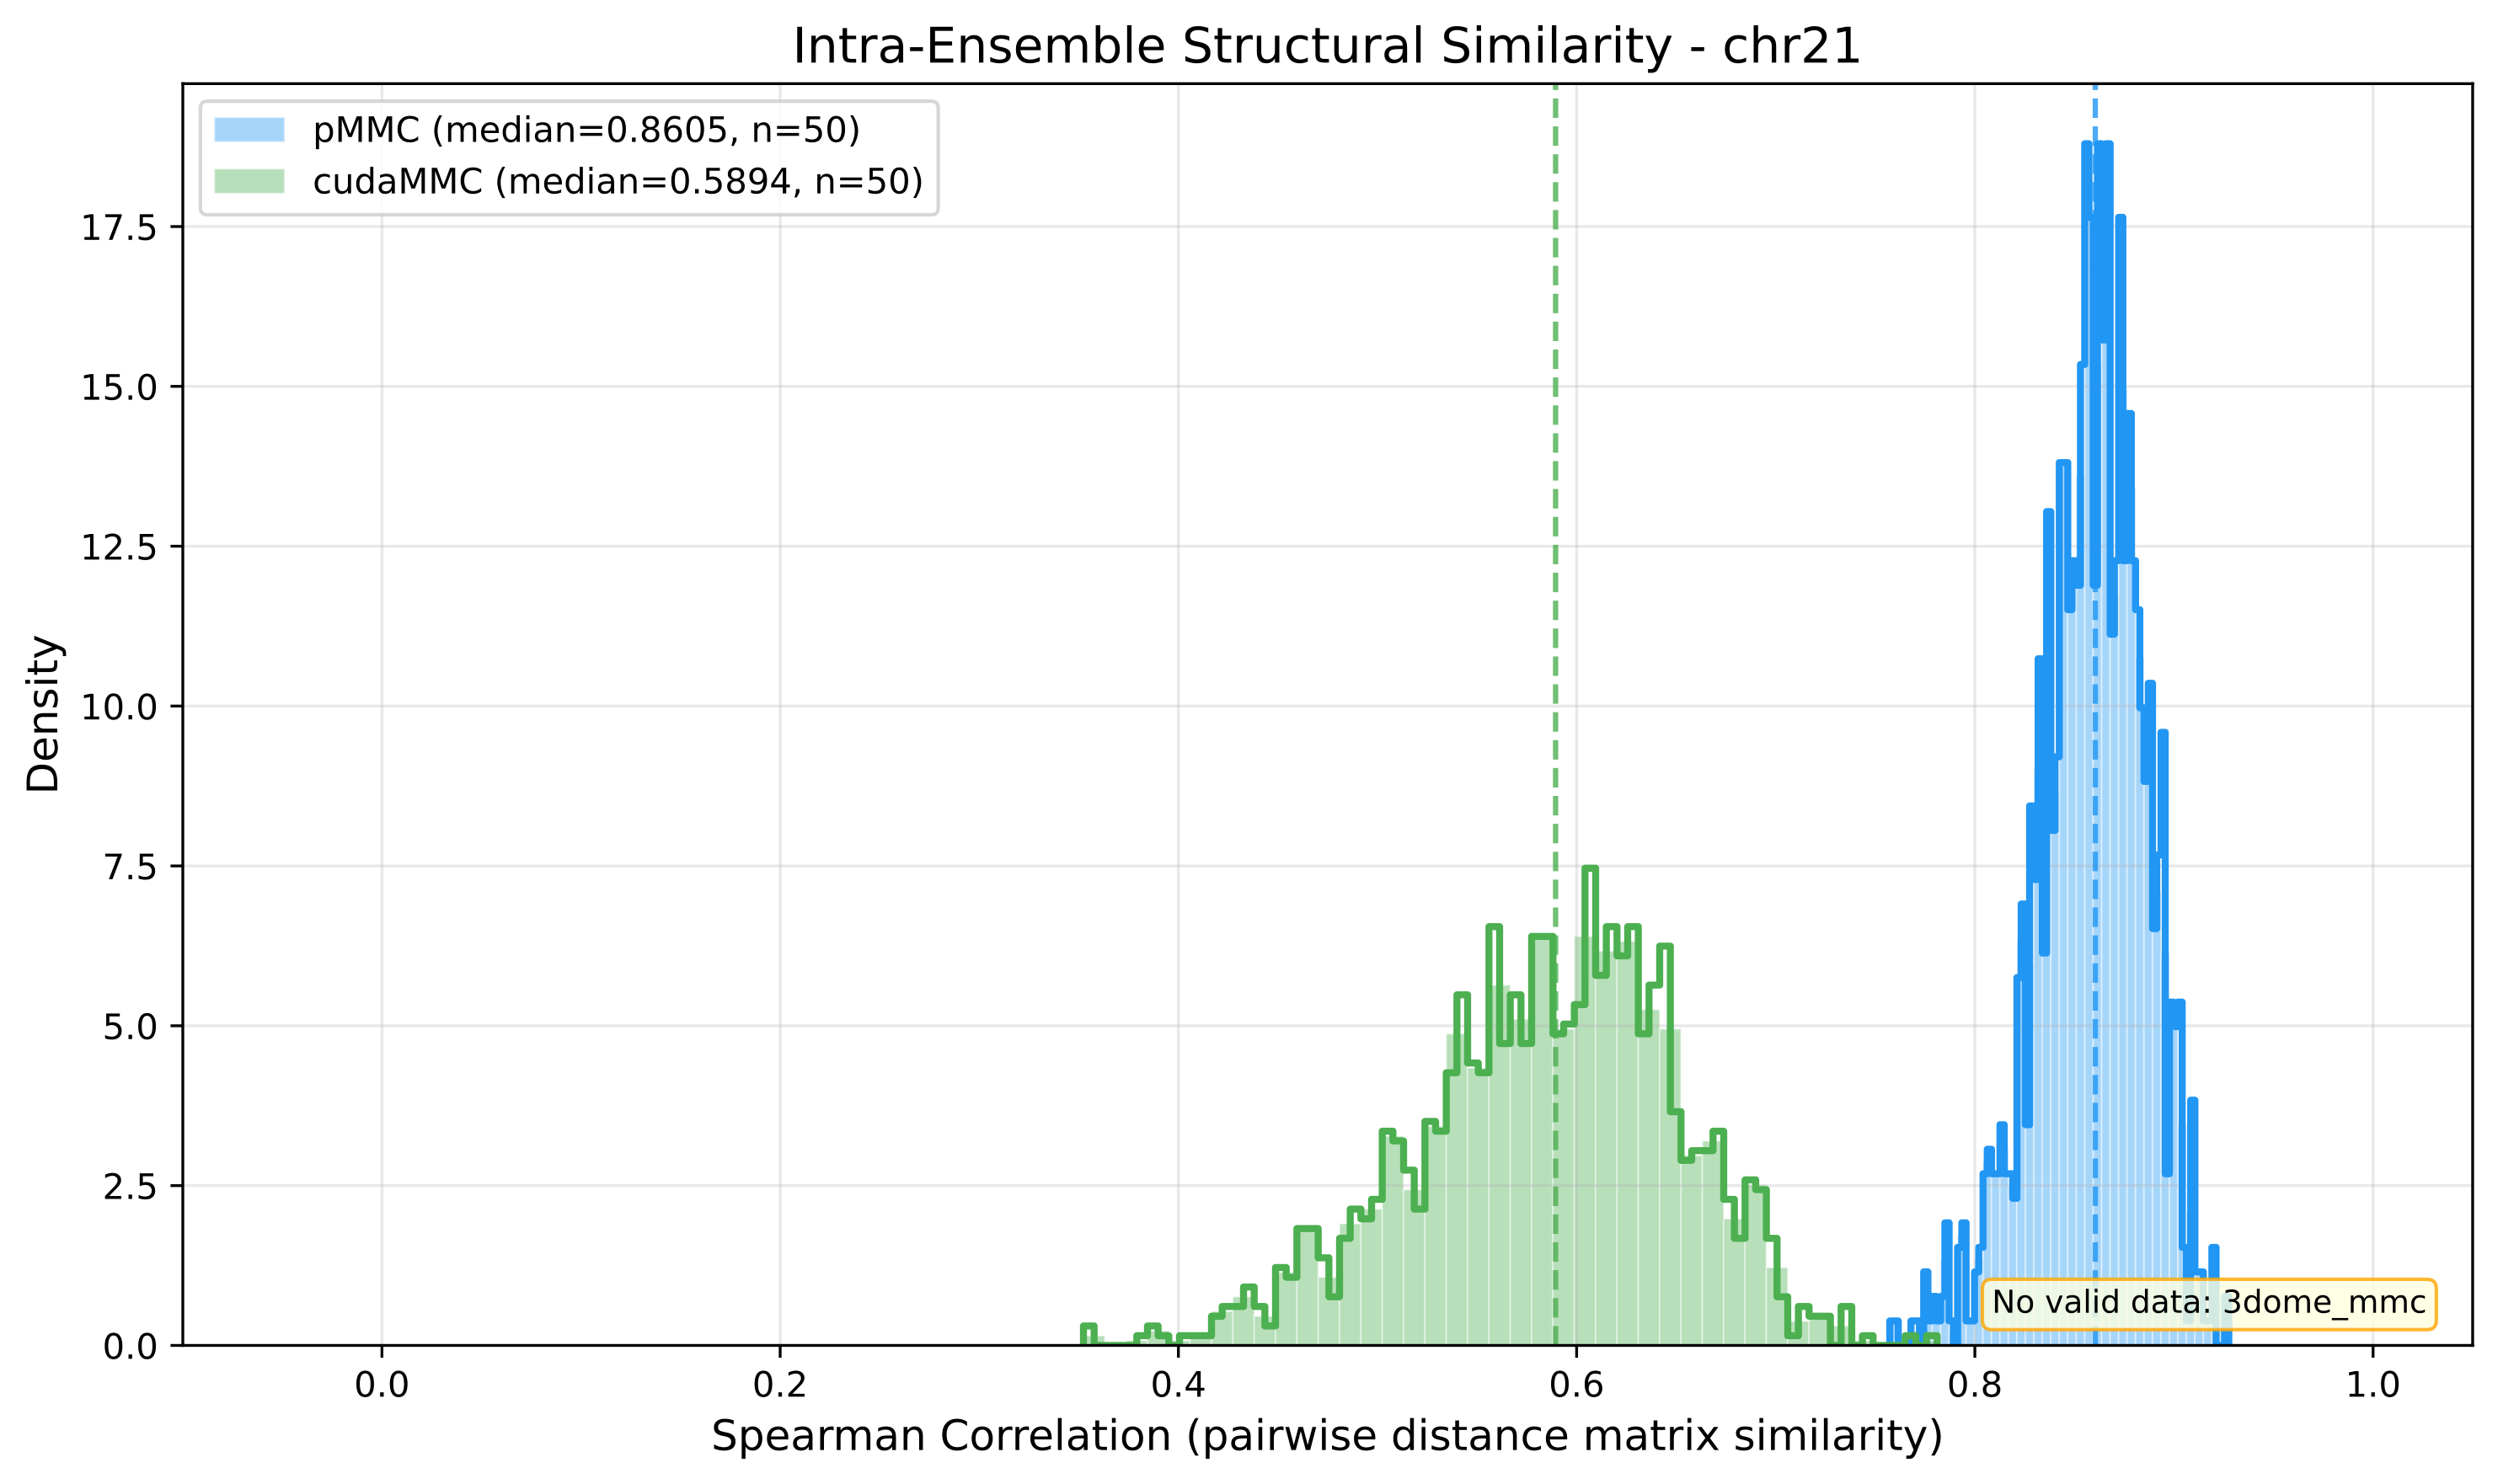
\includegraphics[width=\columnwidth]{similarity_density_chr21.png}
\caption{Pairwise similarity distributions within ensembles of 50 models for chromosome~21. pMMC produces ensembles with higher inter-model consistency (median similarity 0.86, mean 0.86) than cudaMMC (median 0.59, mean 0.58).}\label{fig:similarity}
\end{figure}

\paragraph{Resource utilisation.}
Table~\ref{tab:resources} summarises GPU and memory statistics for chr1. All three tools use comparable peak VRAM (${\sim}\,930$--$1030$\,MiB). Peak system RAM is approximately 107\,MB for pMMC and cudaMMC, versus ${\sim}\,12$\,MB for 3D-GNOME which does not load CUDA libraries. The mean GPU utilisation of pMMC (3.2\%) and cudaMMC (2.4\%) reflects the short burst nature of the GPU kernels; the low sustained utilisation is expected because each kernel runs for only tens to hundreds of milliseconds before returning control to the host for the next interaction block. CPU utilisation decreases from 95.7\% (3D-GNOME) through 63.7\% (cudaMMC) to 40.8\% (pMMC), reflecting the progressive offloading of computational work to the GPU.

\begin{table}[!t]
\caption{Resource utilisation (mean across 10 runs for chr1).\label{tab:resources}}%
\begin{tabular*}{\columnwidth}{@{\extracolsep\fill}lccc@{\extracolsep\fill}}
\toprule
Metric & 3D-GNOME & cudaMMC & pMMC \\
\midrule
Peak RSS (MB)          & 11.8  & 106.7  & 104.6 \\
Peak VRAM (MiB)        & 979.7 & 1028.7 & 930.8 \\
Mean GPU util.\ (\%)   & 3.0   & 2.4    & 3.2   \\
Mean power (W)         & 9.7   & 17.2   & 22.5  \\
CPU util.\ (\%)        & 95.7  & 63.7   & 40.8  \\
\botrule
\end{tabular*}
\end{table}

%% =====================================================================
%% 4. CONCLUSIONS
%% =====================================================================

\section{Conclusions}

We have presented pMMC, a fully GPU-accelerated tool for multiscale Monte Carlo reconstruction of 3D chromatin structures. By transferring all three simulated annealing phases to CUDA kernels and employing a persistent GPU resource cache, pMMC achieves up to 1.52$\times$ speedup over cudaMMC and 13.6$\times$ over the original CPU-based 3D-GNOME, with the advantage growing for larger chromosomes. Output quality is numerically identical to cudaMMC ($r = 1.000$), and 50-model ensembles exhibit higher structural consistency (median Spearman $\rho = 0.86$ vs.\ $0.59$). The near-constant wall-clock time across chromosomes of all sizes makes pMMC particularly well suited for genome-wide modelling and for generating statistical ensembles required by downstream analyses such as promoter--enhancer distance profiling \citep{Wlasnowolski2023gnome}. pMMC further offers multidimensional scaling initialisation, mmCIF/PDB export, and built-in benchmarking with structural comparison metrics. These improvements make pMMC a practical tool for whole-genome-scale 3D structure modelling from ChIA-PET data.

%% =====================================================================
%% BACK-MATTER (verbatim as required)
%% =====================================================================

\section*{Supplementary data}
Supplementary data are available at \textit{Bioinformatics} online.

\section*{Data availability}
The ChIA-PET interaction data used for benchmarking are
available in the project repository. Reconstructed 3D structures
in HCM, mmCIF, and PDB formats are included in the benchmark
output directory.

\section*{Conflict of interest}
None declared.

\section*{Funding}
D.P.\ and K.S.\ research was funded by Warsaw University of Technology within the Excellence Initiative: Research University (IDUB) programme and co-supported by Polish National Science Centre (2020/37/B/NZ2/03757). The work was supported by National Institute of Health USA 4DNucleome grant 1U54DK107967-01 ``Nucleome Positioning System for Spatiotemporal Genome Organization and Regulation''.

\section*{Author contributions statement}
M.N.S.\ implemented pMMC, conducted benchmark
experiments, and drafted the manuscript. K.S.\ supervised the
benchmarking process and reviewed the manuscript. D.P.\ conceived
the project. All authors read and approved the final version.

\section*{Acknowledgments}
Computational resources were provided by M.N.S.'s personal
hardware.

\bibliographystyle{oup-abbrvnat}
\bibliography{references}

\end{document}
